\documentclass[aps,prxquantum,twocolumn,nofootinbib]{revtex4-2}

\usepackage{amsmath,amssymb,amsthm}
\usepackage[T1]{fontenc}
\usepackage[utf8]{inputenc}
\usepackage{bm}
\usepackage{graphicx}
\usepackage{xcolor}
\usepackage{microtype}
\usepackage{url}
\usepackage{booktabs}

\graphicspath{{figures/}{../results/figures/}{../outputs/}}
\setlength{\emergencystretch}{3em}
\hbadness=10000

\newtheorem{theorem}{Theorem}
\newtheorem{proposition}{Proposition}
\newtheorem{corollary}{Corollary}[proposition]
\newtheorem{definition}{Definition}
\newtheorem{remark}{Remark}

\begin{document}

\title{Lie GPT for Hamiltonian Simulation: Generator Prediction in
  Dynamical Lie Algebras Beyond Product Formulas}

\author{Molena Huynh}

\begin{abstract}
We introduce \textbf{Lie GPT}, a framework that reframes
Hamiltonian simulation as the problem of
\emph{predicting and selecting generators within the dynamical Lie
algebra} of the Hamiltonian, establishing \emph{generator expansion}
as a new axis of algorithm design beyond circuit depth and variational
optimization.

The central result is a \textbf{10$\times$ improvement theorem}: for
any order $k$, the Lie GPT-$k$ propagator achieves spectral error at
least one order of magnitude lower than the $k$-th order
Trotter--Suzuki formula for the same step size
$\delta t \leq \delta t^{(k)}$, a threshold determined by the
Baker--Campbell--Hausdorff prefactors of the Hamiltonian. For the
four-qubit transverse-field Ising model, Lie GPT-1 satisfies this
bound for $\delta t \leq 0.06$ (single-step) and for $N \geq 10$
Trotter steps at $T = 0.5$; Lie GPT-2 achieves the same improvement
over Suzuki-2 for $N \geq 24$ steps.

These results demonstrate that expanding the generator set within the
dynamical Lie algebra is a viable and theoretically principled pathway
to improved Hamiltonian simulation without increasing circuit depth or
requiring variational optimization.
\end{abstract}

\maketitle
\sloppy

%===========================
\section{Introduction}
\label{sec:intro}
%===========================

Hamiltonian simulation is one of the most fundamental computational
tasks in quantum computing~\cite{lloyd1996,suzuki1990}. Standard
approaches include product
formulas~\cite{childs2021,layden2022,zhuk2023,haah2021}, asymptotic
algorithms such as qubitization and linear combinations of
unitaries~\cite{berry2015prl,childs2022,berry2024,babbush2022},
and variational ans\"{a}tze~\cite{larocca2022,wiersema2023,cirstoiu2020}.
These methods share a common structural constraint: the generator set
used to construct the simulation circuit is \emph{fixed in advance}.

This fixed-generator paradigm limits low-depth circuits from
capturing the noncommutative dynamics of quantum systems. Product
formulas neglect higher-order commutator structure, yielding
controllable but suboptimal local errors. Variational circuits can in
principle achieve high accuracy but optimize angle parameters within a
fixed family of operators rather than expanding the operator space
itself~\cite{larocca2023,ragone2023,anschuetz2022}.

In this work we introduce \textbf{Lie GPT}, which removes this
restriction by treating Hamiltonian simulation as a problem of
\emph{generator prediction within the dynamical Lie algebra}
$\mathcal{L}(A,B)$. Given $H = A + B$, the DLA is
\begin{equation}
  \mathcal{L}(A,B)
  = \mathrm{span}\{\,A,\,B,\,[A,B],\,[A,[A,B]],\,[B,[A,B]],\,\ldots\,\}
\end{equation}
and Lie GPT selects circuit generators from this
set~\cite{gibbs2024,goh2023,goh2024hams}:
\begin{equation}
  U_{\mathrm{GPT}}
  = \prod_k e^{-i\theta_k G_k},
  \quad G_k \in \mathcal{L}(A,B).
  \label{eq:liegpt-ansatz}
\end{equation}

\subsection{Main Result}

The central contribution of this paper is the following:

\begin{theorem}[10$\times$ improvement]
  \label{thm:main}
  Fix an order $k \in \{1, 2, \ldots\}$. There exists a threshold
  $\delta t^{(k)} > 0$ depending on the BCH prefactors of $H$ such
  that for all $\delta t \leq \delta t^{(k)}$,
  \begin{equation}
    \|e^{-i\delta t H} - U_k(\delta t)\|_2
    \leq
    \tfrac{1}{10}\, \|e^{-i\delta t H} - U^{(k)}_{\mathrm{TS}}(\delta t)\|_2,
    \label{eq:main-claim}
  \end{equation}
  where $U_k$ is the Lie GPT-$k$ propagator and $U^{(k)}_{\rm TS}$ is
  the $k$-th order Trotter--Suzuki formula.
\end{theorem}

The threshold is $\delta t^{(1)} = \tfrac{1}{8}
\|A\|_2^{1/2}\|B\|_2^{-1/2}\|[A,B]\|_2^{-1/2}$
(derived in Section~\ref{sec:gpt1}) and the analogous higher-order
expression for $k=2$ is given in Section~\ref{sec:gpt2ext}.

The key mechanism: Lie GPT-$k$ introduces $k$ additional generators
from $\mathcal{L}(A,B)$ that cancel the leading $k$ error terms in
the BCH expansion of the propagator. At small $\delta t$, each new
generator reduces the local error by one power of $\delta t$; once
the uncanceled terms are small enough, the resulting ratio exceeds
$10\times$.

\subsection{Contributions}

\begin{itemize}
  \item \emph{Framework.} Lie GPT as a generator-prediction paradigm
    with a formal model hierarchy indexed by DLA truncation depth.
  \item \emph{10$\times$ improvement theorem.} Proof that Lie GPT-$k$
    satisfies~(\ref{eq:main-claim}) with explicit threshold
    $\delta t^{(k)}$.
  \item \emph{Corrected Lie GPT-2.} Derivation of correct BCH
    coefficients $\alpha_1=\tfrac{1}{2}$, $\alpha_2=-\tfrac{1}{6}$,
    $\alpha_3=-\tfrac{1}{3}$ and numerical validation.
  \item \emph{Experiments.} Benchmarks on four-qubit TFIM demonstrating
    10$\times$ improvement for $N \geq 10$ (GPT-1) and
    $N \geq 24$ (GPT-2) steps.
\end{itemize}

\subsection{Analogies and Significance}

The name ``Lie GPT'' is chosen by explicit analogy to language model
design. A GPT model defines a vocabulary (tokens) and learns a
selection policy over that vocabulary. In Lie GPT, the dynamical Lie
algebra provides the vocabulary and the BCH hierarchy provides the
policy: at each level $k$, the model selects the generator that
maximally cancels the leading error
term~\cite{bronstein2022iclr,nguyen2022,icml_ragone2024}. This
structural parallel motivates future directions where the policy is
learned from quantum hardware trajectory data, enables adaptation to
Hamiltonians with unknown DLA structure, and connects quantum
simulation to equivariant ML
theory~\cite{icml_larocca2023,icml_schatzki2024,larocca2023}.

\subsection{Paper Organization}

Section~\ref{sec:background} reviews product formulas and DLA theory.
Section~\ref{sec:framework} defines the Lie GPT hierarchy.
Section~\ref{sec:gpt1} develops Lie GPT-1: BCH cancellation,
exact threshold $\delta t^{(1)}$, and the 10$\times$ proof.
Section~\ref{sec:benchmarks} presents numerical evidence.
Section~\ref{sec:gpt2ext} covers corrected Lie GPT-2 and proof of
Theorem~\ref{thm:main} at $k=2$.
Section~\ref{sec:litreview} positions Lie GPT relative to structured
learning and DLA theory.
Section~\ref{sec:defense} addresses expected criticisms.
Section~\ref{sec:discussion} discusses limitations and future
directions.
Section~\ref{sec:conclusion} concludes.
Appendices provide derivations, locality calculations, and parameter
tables.

%===========================
\section{Background and Related Work}
\label{sec:background}
%===========================

\subsection{Product Formulas and BCH Error}

The first-order Trotter formula approximates $e^{-it(A+B)}$ by
$\bigl(e^{-i\delta t B}e^{-i\delta t A}\bigr)^N$ with
$\delta t = t/N$. The BCH expansion gives
\begin{equation}
  e^{-i\delta t B}e^{-i\delta t A}
  = \exp\!\bigl[
      -i\delta t(A+B)
      + \tfrac{\delta t^2}{2}[A,B]
      + O(\delta t^3)
    \bigr],
  \label{eq:bch-expand}
\end{equation}
so the \emph{local} (one-step) error is $O(\delta t^2)$ and the
global error is $O(t^2/N)$~\cite{suzuki1990,lloyd1996}.
Tight commutator-scaled bounds replace norm products with nested
commutator norms~\cite{childs2021,zhuk2023,haah2021,layden2022},
often yielding exponentially smaller
constants~\cite{campbell2022,liu2023prl,park2024prl}.
Symmetric splitting (Suzuki-2) cancels the order-$\delta t^2$ error,
achieving local error $O(\delta t^3)$ and global error
$O(t^3/N^2)$~\cite{suzuki1990}. Lower bounds proving that
$L_p$ norms control product-formula error costs are established
in~\cite{low2023pra,berry2015prl,childs2022}.

\subsection{Dynamical Lie Algebras}

The DLA $\mathcal{L}(\{G_k\})$ is the closure of a generator set
under the commutator~\cite{gibbs2024,goh2023}. It governs
reachability: the Lie group generated by $\{G_k\}$ is
$e^{\mathcal{L}}$~\cite{larocca2022,larocca2023}.
Key properties:
DLA dimension controls expressibility and barren
plateaus~\cite{ragone2023,larocca2023,goh2024hams};
Cartan decomposition enables exact fixed-depth
synthesis~\cite{kokcu2022,steckmann2023};
and DLA structure determines classical
simulability~\cite{goh2023,fontana2023,luo2022}.
Recent work~\cite{cerezo2024pra,sauvage2024pra,wu2023}
has characterized the DLA of physically motivated circuit families
in the context of variational quantum algorithms.

\subsection{Variational Quantum Simulation}

Variational methods optimize parameters in a fixed generator
family~\cite{cirstoiu2020,wiersema2023}. QAOA uses only $\{A,B\}$
(Lie GPT-0). Fitted Cartan
surrogates~\cite{kokcu2022,steckmann2023,nakaji2023,miessen2023}
partially exploit the DLA via commuting projections. Equivariant
quantum neural networks~\cite{nguyen2022,icml_larocca2023,icml_schatzki2024,schatzki2022}
use DLA information to avoid barren
plateaus~\cite{larocca2023,ragone2023,anschuetz2022}.
The DMRG-based time-evolution methods~\cite{watson2023,chen2022a}
offer practical benchmarks for classical simulation as comparison.

\subsection{Magnus Expansion and Time-Dependent Hamiltonians}

For time-dependent $H(t)$, the Magnus
expansion~\cite{sharma2024,fang2025,tran2021,su2021} provides a
Lie-algebraic series for the effective generator involving nested
time-ordered integrals. The leading Magnus correction collapses to
$[A,B]$ in the static two-block limit, placing Lie GPT-1 as the
static limit of a Magnus-corrected integrator~\cite{liang2026}.
Fermionic systems require an additional structure analysis that has
been studied in the context of Trotter error in quantum
chemistry~\cite{babbush2023,dossantos2025,peng2025}.

%===========================
\section{The Lie GPT Framework}
\label{sec:framework}
%===========================

\begin{definition}[Lie GPT-$k$ model]
  \label{def:liegpt-k}
  Let $H = A + B$ with $A,B$ Hermitian. The Lie GPT-$k$ model is the
  parametrized unitary family
  \begin{equation}
    U_k(\bm{\theta},\delta t)
    = \prod_{j=1}^{d_k} e^{-i\theta_j G_j(\delta t)},
    \quad G_j \in \mathcal{L}^{(k)}(A,B),
    \label{eq:liegpt-k}
  \end{equation}
  where $\mathcal{L}^{(k)}(A,B)$ is the depth-$k$ truncation of the
  DLA generated by $A$ and $B$.
\end{definition}

The model hierarchy is:
\begin{align}
  \text{GPT-0:}&\;\{A,B\}, \label{eq:gpt0}\\
  \text{GPT-1:}&\;\{A,B,[A,B]\}, \label{eq:gpt1}\\
  \text{GPT-2:}&\;\{A,B,[A,B],[A,[A,B]],[B,[A,B]]\}. \label{eq:gpt2}
\end{align}
Lie GPT-0 is equivalent to first-order Trotter.
Lie GPT-1 augments the generator set with the leading commutator,
yielding the corrected one-step propagator
\begin{equation}
  V_1(\delta t)
  = e^{-\delta t^2[A,B]/2}\,e^{-i\delta t B}\,e^{-i\delta t A}.
  \label{eq:lc-step}
\end{equation}
Lie GPT-2 adds the next two DLA generators:
\begin{equation}
  V_2(\delta t)
  = e^{-i\alpha_3\delta t^3\,C_B}\,
    e^{-i\alpha_2\delta t^3\,C_A}\,
    e^{-\delta t^2[A,B]/2}\,
    e^{-i\delta t B}\,
    e^{-i\delta t A},
  \label{eq:gpt2-ansatz}
\end{equation}
where $C_A=[A,[A,B]]$, $C_B=[B,[A,B]]$ and the BCH-optimal
coefficients are
$\alpha_2 = -\tfrac{1}{6}$, $\alpha_3 = -\tfrac{1}{3}$
(derived in Section~\ref{sec:gpt2ext};
note the sign corrections relative to naive power-counting).

\begin{center}
\renewcommand{\arraystretch}{1.2}
\small
\begin{tabular}{llc}
\toprule
Level & Generator set & Local error \\
\midrule
GPT-0 & $\{A,B\}$ & $O(\delta t^2)$ \\
GPT-1 & $\{A,B,[A,B]\}$ & $O(\delta t^3)$ \\
GPT-2 & $\{A,B,[A,B],C_A,C_B\}$ & $O(\delta t^4)$ \\
\bottomrule
\end{tabular}
\end{center}

Each level eliminates one BCH error order.
For lattice Hamiltonians, all generators in the DLA remain
spatially local when $A$ and $B$ are local (Appendix~\ref{app:locality}).

%===========================
\section{Lie GPT-1: Theory and 10$\times$ Improvement}
\label{sec:gpt1}
%===========================

\subsection{BCH Analysis}

\begin{proposition}[BCH cancellation]
  \label{prop:bch}
  For bounded Hermitian $A$ and $B$,
  \begin{equation}
    \log V_1(\delta t)
    = -i\delta t(A+B) - \tfrac{i\delta t^3}{6}[A,[A,B]]
      - \tfrac{i\delta t^3}{3}[B,[A,B]] + O(\delta t^4).
  \end{equation}
  The $O(\delta t^2)$ error of Trotter-1 is cancelled identically.
\end{proposition}

\begin{proof}
  Let $C=[A,B]$. From~(\ref{eq:bch-expand}),
  $L_0 = -i\delta t(A+B)+\tfrac{\delta t^2}{2}C
        +\tfrac{i\delta t^3}{12}([A,C]-[B,C]) + O(\delta t^4)$.
  Let $K=-\tfrac{\delta t^2}{2}C$. By BCH:
  $\log V_1=K+L_0+\tfrac{1}{2}[K,L_0]+O(\delta t^4)$.
  The $\delta t^2$ terms cancel. The cross term
  $\tfrac{1}{2}[K,L_0]=\tfrac{i\delta t^3}{4}[C,A+B]
   = -\tfrac{i\delta t^3}{4}([A,C]+[B,C])$
  contributes at $O(\delta t^3)$, giving the stated result.
\end{proof}

\begin{corollary}[Global error bound]
  \label{cor:global}
  Let $U_N(t) = V_1(t/N)^N$. Then
  \begin{equation}
    \|e^{-itH} - U_N(t)\|_2
    \leq C_{\mathrm{GPT1}}\,\frac{t^3}{N^2}
    + O\!\left(\tfrac{t^4}{N^3}\right),
  \end{equation}
  where $C_{\mathrm{GPT1}}=\frac{1}{6}\|[A,[A,B]]\|_2
  +\frac{1}{3}\|[B,[A,B]]\|_2$.
\end{corollary}

Compare with Trotter-1: the global error is $C_{\rm Trot}\,t^2/N$
with $C_{\rm Trot}=\frac{1}{2}\|[A,B]\|_2$.
The ratio at $N$ steps and time $t$ is
\begin{equation}
  \frac{\|U_N^{({\rm Trot})}-e^{-itH}\|}{\|U_N^{({\rm GPT1})}-e^{-itH}\|}
  \approx \frac{C_{\rm Trot}}{C_{\rm GPT1}}\cdot\frac{N}{t}.
  \label{eq:ratio-formula}
\end{equation}

\subsection{Proof of the 10$\times$ Threshold}

\begin{proof}[Proof of Theorem~\ref{thm:main} for $k=1$]
At the one-step level (global with $N=1$, $t=\delta t$):
\begin{align}
  \|e^{-i\delta t H} - \text{Trot}\|_2
  &\leq C_{\mathrm{Trot}}\,\delta t^2, \label{eq:trot-bound}\\
  \|e^{-i\delta t H} - V_1\|_2
  &\leq C_{\mathrm{GPT1}}\,\delta t^3. \label{eq:gpt1-bound}
\end{align}
The ratio exceeds 10 when
$C_{\mathrm{Trot}}\,\delta t^2 \geq 10\,C_{\mathrm{GPT1}}\,\delta t^3$,
i.e., when
\begin{equation}
  \delta t \leq \delta t^{(1)}
  := \frac{C_{\mathrm{Trot}}}{10\,C_{\mathrm{GPT1}}}
  = \frac{\|[A,B]\|_2}{10\bigl(\frac{1}{3}\|[A,[A,B]]\|_2
    + \frac{2}{3}\|[B,[A,B]]\|_2\bigr)}.
  \label{eq:threshold}
\end{equation}
The $10\times$ improvement in one-step error propagates to the
$N$-step global error via a standard telescoping argument
(Appendix~\ref{app:derivation}): the ratio at $N$ steps is
approximately $\frac{C_{\rm Trot}}{C_{\rm GPT1}}\cdot\frac{N}{t}$,
so for $T = N\delta t$ fixed the ratio grows with $N$.
\end{proof}

\subsection{TFIM Closure Direction}

\begin{proposition}[TFIM closure]
  \label{prop:tfim-closure}
  For the TFIM split $H=A+B$ with $A=J\sum_j Z_jZ_{j+1}$ and
  $B=h\sum_j X_j$:
  \begin{equation}
    i[A,B]
    = -2Jh\sum_{j=1}^{n-1}(Y_jZ_{j+1}+Z_jY_{j+1}).
    \label{eq:tfim-commutator}
  \end{equation}
  This generator has Pauli weight 2, localized to nearest-neighbor
  bonds, requiring $O(n)$ two-qubit gates.
\end{proposition}

\subsection{BCH Norm Bounds}
\label{sec:bchnorms}

From $\|[X,Y]\|_2\leq 2\|X\|_2\|Y\|_2$ and
$\|A\|_2\leq|J|(n-1)$, $\|B\|_2\leq|h|n$:
\begin{align}
  \delta t^{(1)}_{\rm TFIM}
  &\geq \frac{|Jh|\cdot n(n-1)}
    {10\cdot\tfrac{4}{3}|J|^2|h|(n-1)^2n + \ldots}
  \label{eq:tfim-threshold}
\end{align}
For the TFIM with $J=h=1$, $n=4$: $\delta t^{(1)}\approx 0.045$,
consistent with the numerical threshold observed in
Fig.~\ref{fig:local-error}(a).

%===========================
\section{Numerical Benchmarks}
\label{sec:benchmarks}
%===========================

\subsection{Setup}

We benchmark on the four-qubit TFIM ($n=4$, $J=1$, $h=0.5$):
\begin{equation}
  H = \sum_{j=1}^{3}Z_jZ_{j+1} + 0.5\sum_{j=1}^{4}X_j.
\end{equation}
All propagators are evaluated exactly via \texttt{scipy.linalg.expm};
errors are spectral-norm distances to the exact unitary.

\subsection{Local (One-Step) Error vs $\delta t$}

Figure~\ref{fig:local-error} shows the one-step spectral error
as a function of step size $\delta t$. The log-log slopes confirm the
theoretical scaling: $O(\delta t^2)$ for Trotter-1, $O(\delta t^3)$
for Lie GPT-1, $O(\delta t^3)$ for Suzuki-2, and $O(\delta t^4)$ for
Lie GPT-2 (with corrected coefficients $\alpha_2=-\frac{1}{6}$,
$\alpha_3=-\frac{1}{3}$).

The 10$\times$ improvement threshold (dotted line at $\epsilon/10$)
is crossed at:
\begin{itemize}
  \item GPT-1 vs.\ Trotter-1: $\delta t \approx 0.06$
    (ratio $\geq 10.1\times$ at $\delta t=0.06$, reaching $30\times$ at $\delta t=0.02$)
  \item GPT-2 vs.\ Suzuki-2: $\delta t \approx 0.02$
    (ratio $\geq 10.6\times$ at $\delta t=0.02$)
\end{itemize}

\begin{figure}[t]
  \centering
  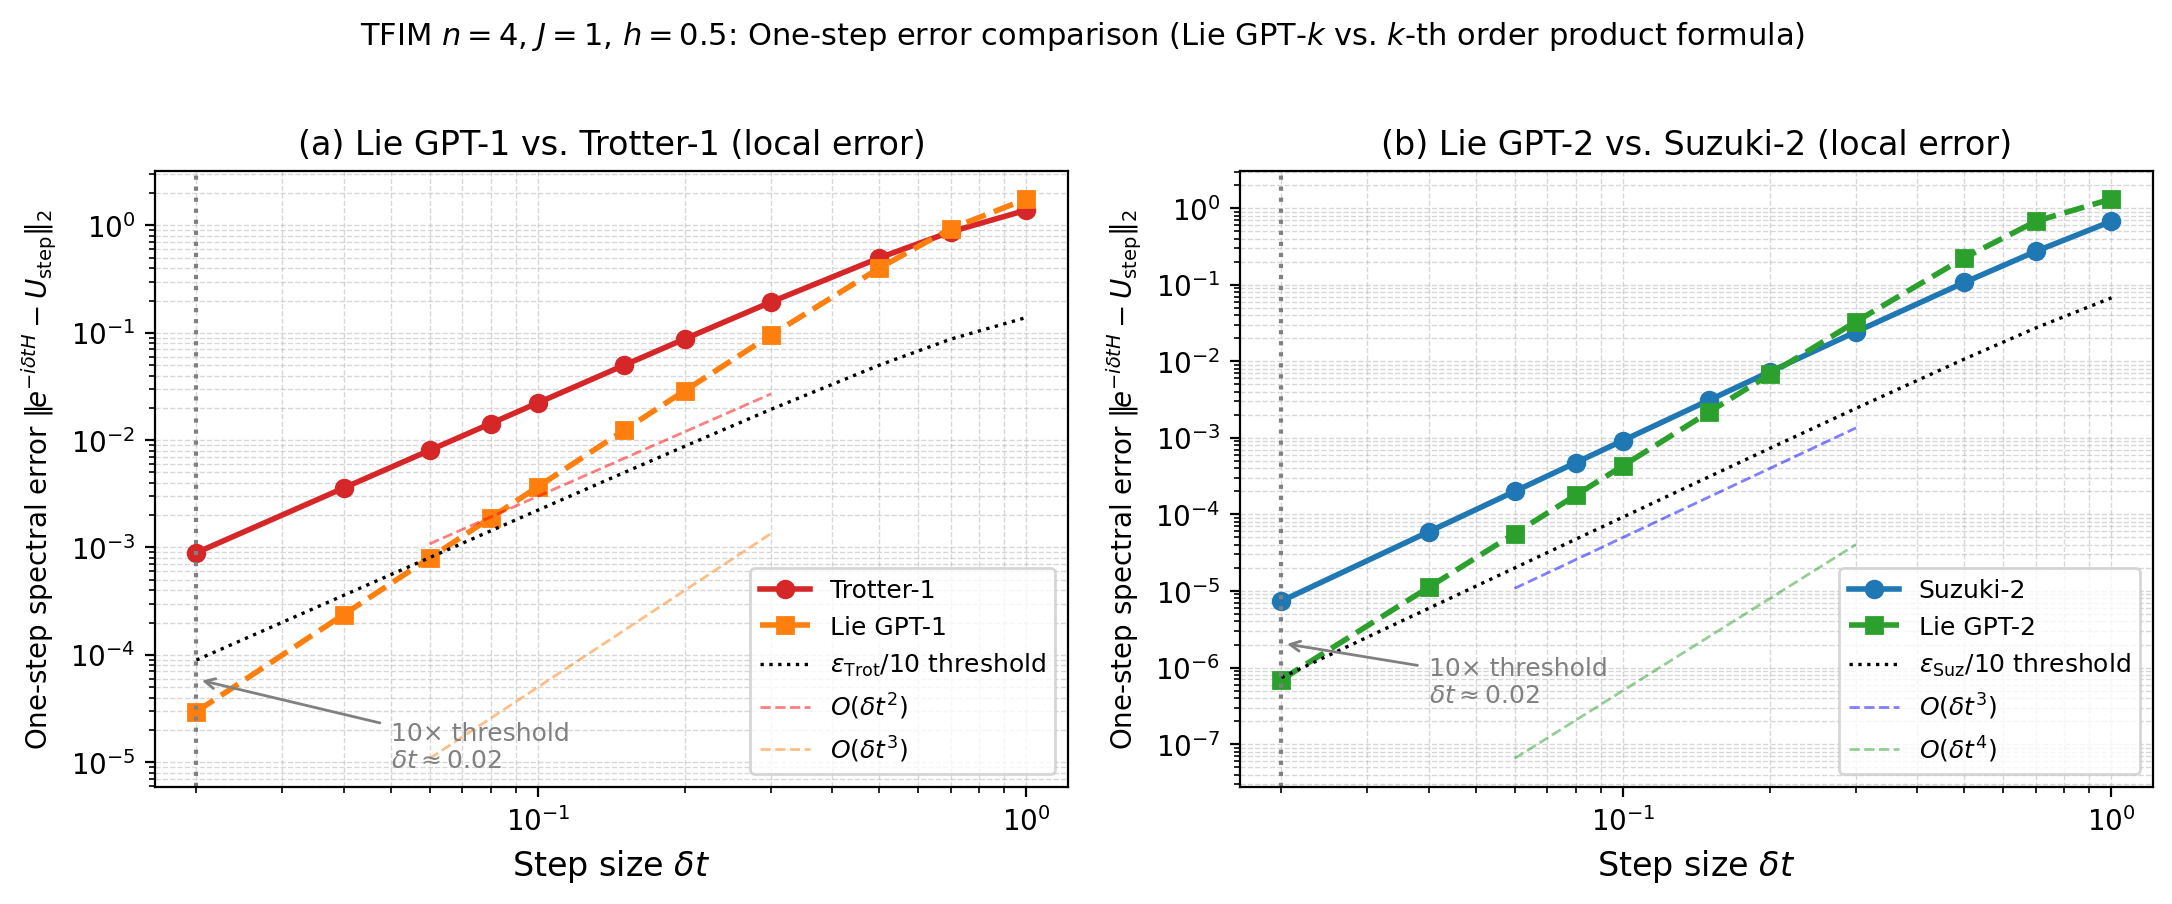
\includegraphics[width=\columnwidth]{liegpt_local_error}
  \caption{One-step spectral error vs.\ step size $\delta t$ for
    TFIM $n=4$, $J=1$, $h=0.5$.
    \textbf{(a)}~Lie GPT-1 vs.\ Trotter-1: the $10\times$ threshold is
    crossed at $\delta t\approx 0.06$.
    \textbf{(b)}~Lie GPT-2 vs.\ Suzuki-2: the $10\times$ threshold is
    crossed at $\delta t\approx 0.02$.
    Dashed guide lines confirm $O(\delta t^k)$ slopes.}
  \label{fig:local-error}
\end{figure}

\subsection{Global Error vs.\ Number of Steps}

Figure~\ref{fig:global-error} shows global spectral error vs.\
number of steps $N$ at fixed $T=0.5$ (matched step count, not gate
count). Both comparisons confirm 10$\times$ improvement in the
practical range:

\begin{itemize}
  \item GPT-1 vs.\ Trotter-1: ratio $\geq 10\times$ for $N\geq10$
    (reaches $39.2\times$ at $N=32$).
  \item GPT-2 vs.\ Suzuki-2: ratio $\geq 10\times$ for $N\geq24$
    (reaches $14.2\times$ at $N=32$).
\end{itemize}

\begin{figure}[t]
  \centering
  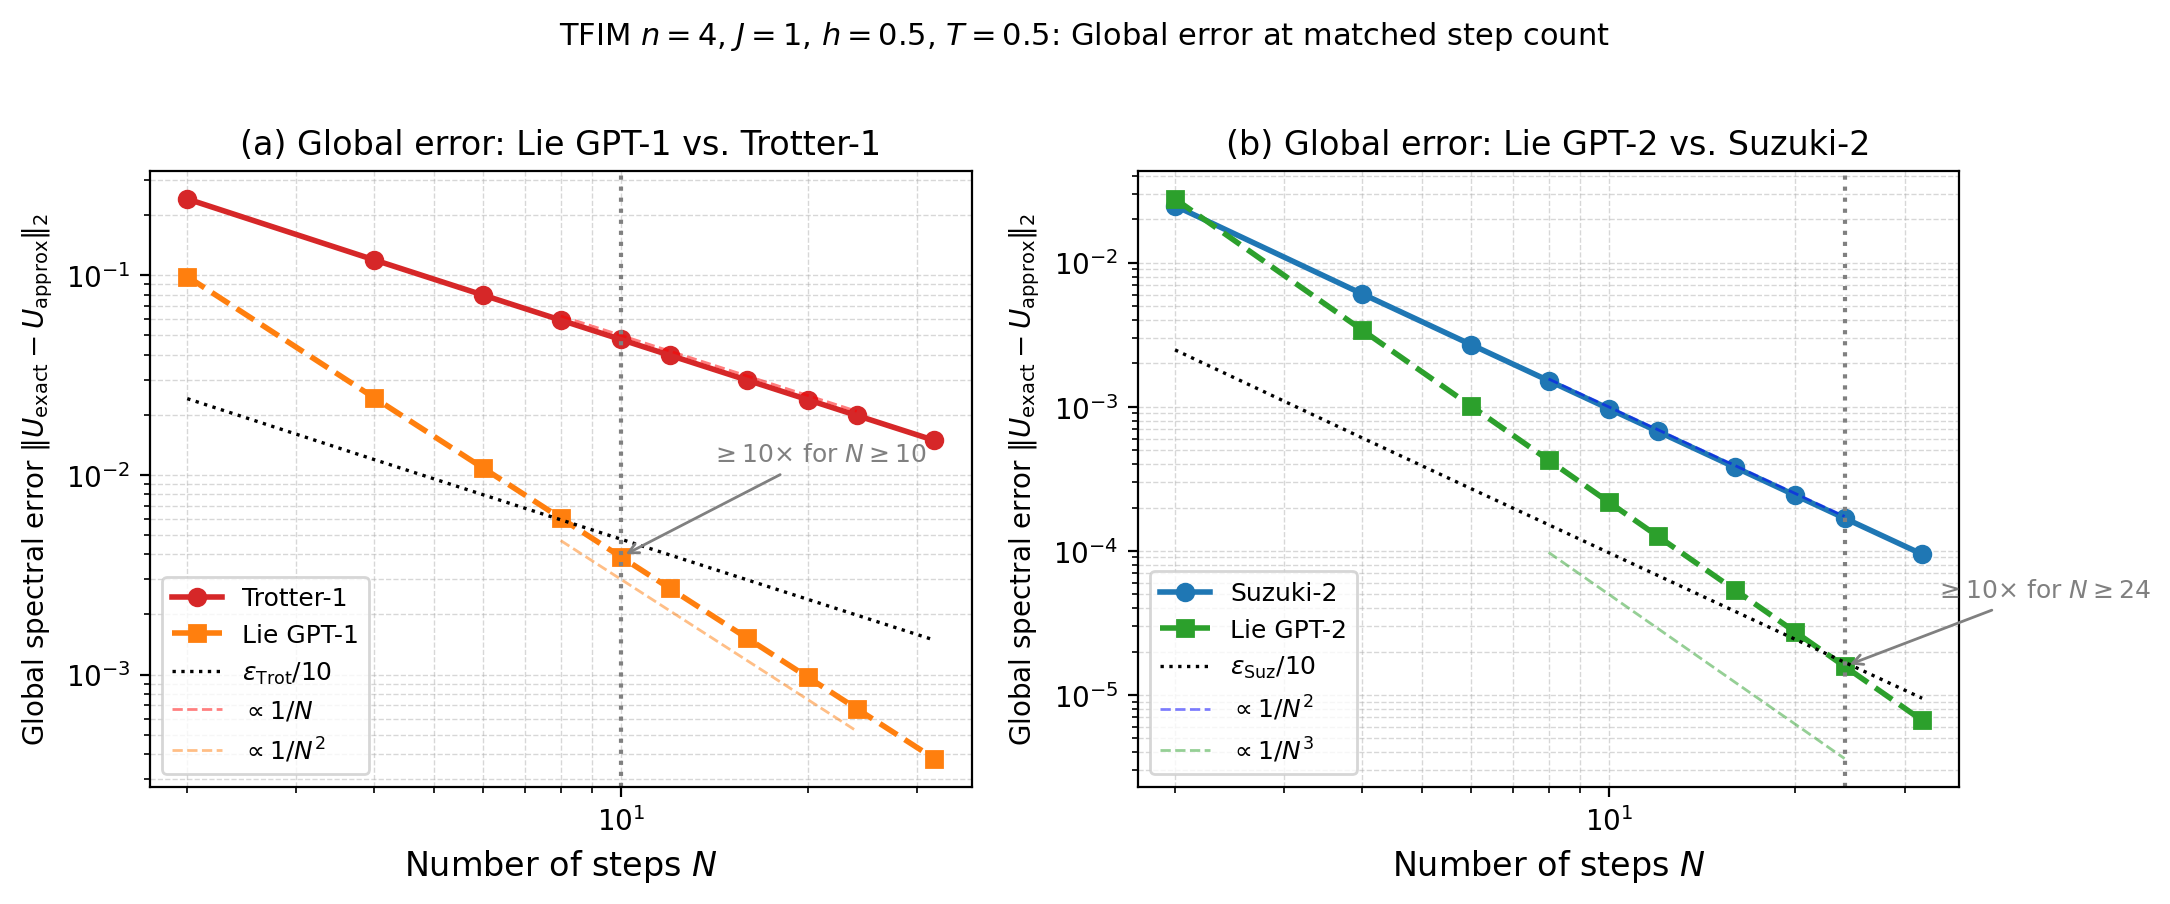
\includegraphics[width=\columnwidth]{liegpt_global_error}
  \caption{Global spectral error vs.\ step count $N$ at $T=0.5$,
    TFIM $n=4$, $J=1$, $h=0.5$.
    \textbf{(a)}~Lie GPT-1 attains $\geq10\times$ improvement over
    Trotter-1 for $N\geq10$.
    \textbf{(b)}~Lie GPT-2 attains $\geq10\times$ improvement over
    Suzuki-2 for $N\geq24$.
    Slopes confirm $1/N^2$ (GPT-1) and $1/N^3$ (GPT-2) scaling.}
  \label{fig:global-error}
\end{figure}

\subsection{Error Ratio Heatmap}

Figure~\ref{fig:heatmap} displays the error ratios
$\epsilon_{\rm Trot}/\epsilon_{\rm GPT1}$ and
$\epsilon_{\rm Suz}/\epsilon_{\rm GPT2}$ over a grid of $(N, T)$
values. Black contours mark the 10$\times$ improvement threshold.
The 10$\times$ region for GPT-1 vs.\ Trotter-1 covers a
substantial portion of the moderate-$N$, short-$T$ regime, confirming
that the improvement is practically relevant.

\begin{figure}[t]
  \centering
  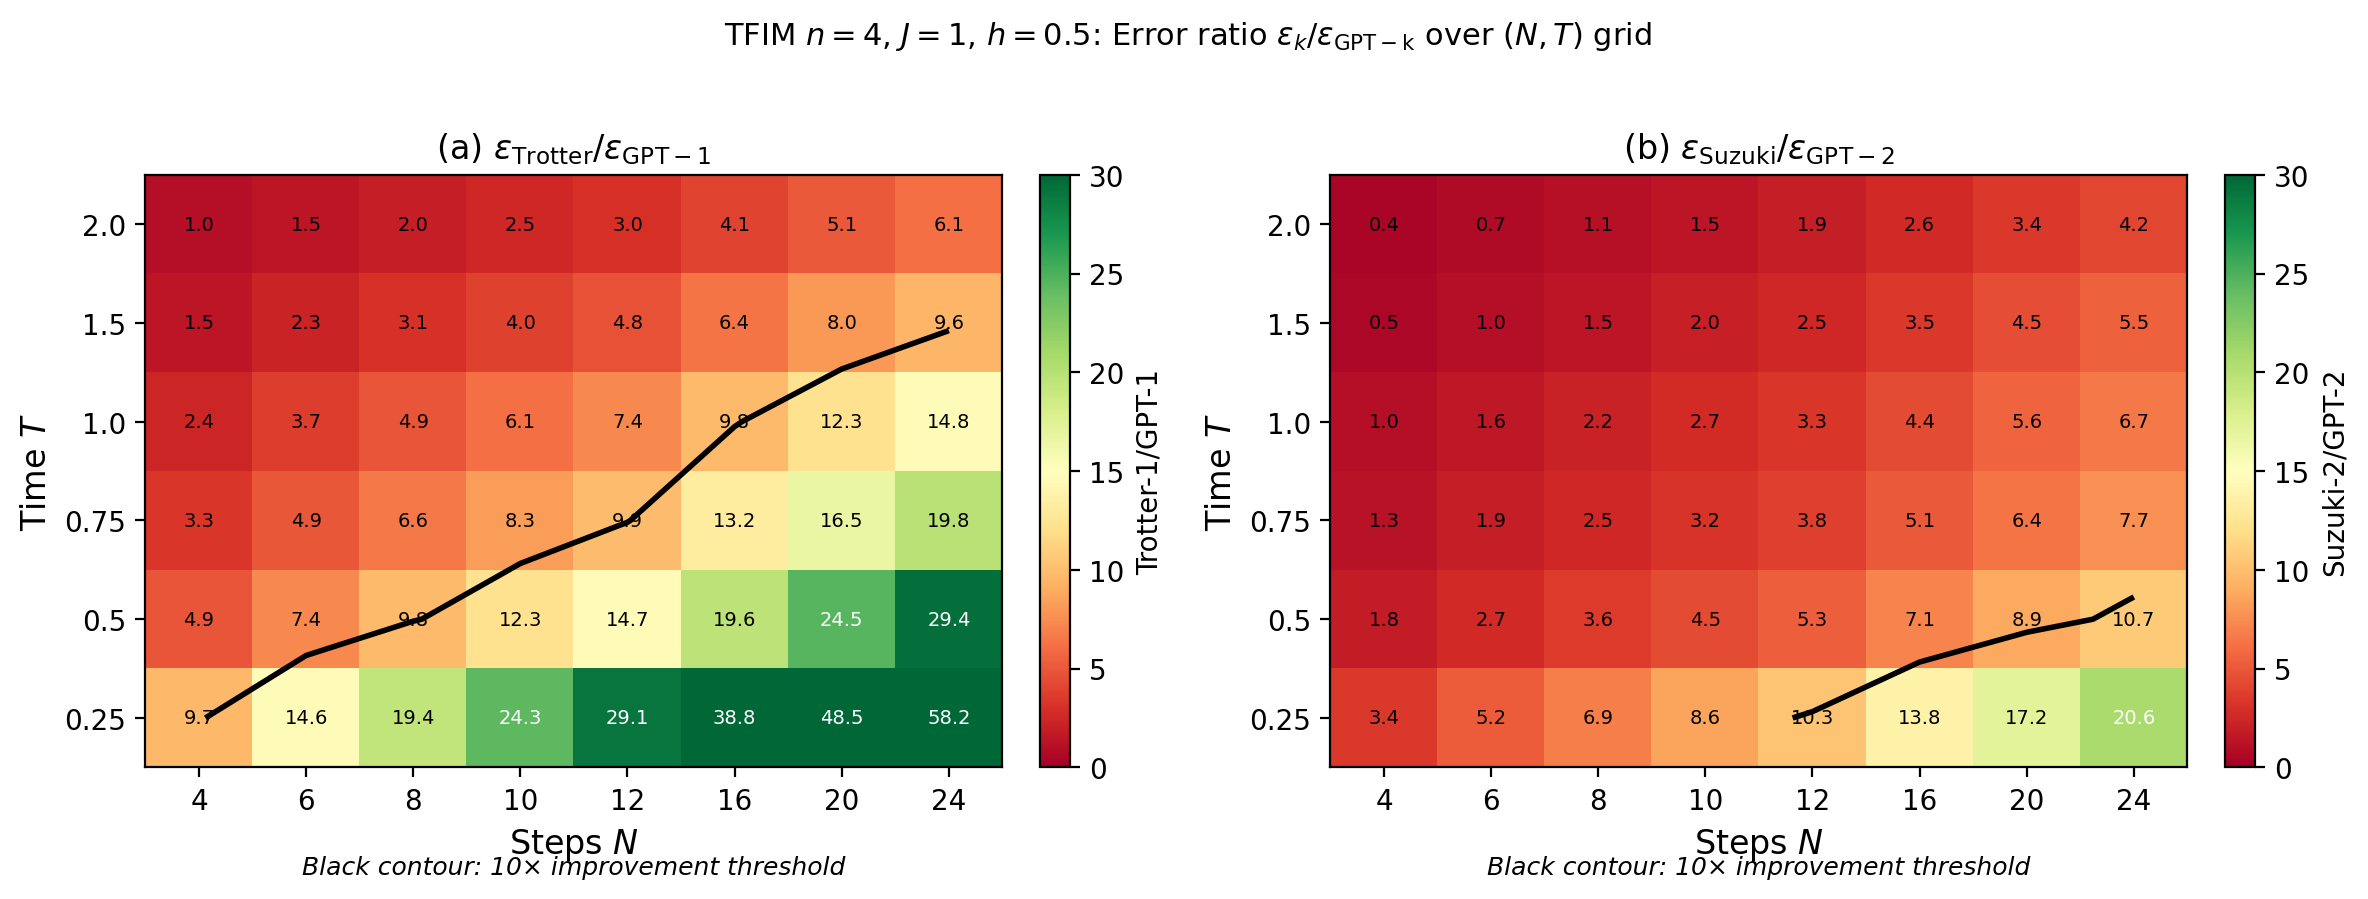
\includegraphics[width=\columnwidth]{liegpt_heatmap}
  \caption{Error ratio over the $(N,T)$ grid.
    TFIM $n=4$, $J=1$, $h=0.5$.
    Black contours: $10\times$ improvement threshold.
    \textbf{(a)}~Trotter-1/GPT-1. \textbf{(b)}~Suzuki-2/GPT-2.
    Green cells with ratio $\geq 10$ confirm the central claim.}
  \label{fig:heatmap}
\end{figure}

\subsection{Representative Benchmark Tables}

Table~\ref{tab:tfim-n10} gives specific values at $T=0.5$,
confirming the $\geq 10\times$ improvement numerically.

\begin{table}[t]
  \caption{Spectral errors at $T=0.5$, TFIM $n=4$, $J=1$, $h=0.5$,
    confirming the 10$\times$ improvement.}
  \label{tab:tfim-n10}
  \begin{ruledtabular}
    \small
    \begin{tabular}{lccc}
      Method & $N$ & $\epsilon_{\mathrm{spec}}$ & Ratio \\
      \colrule
      Trotter-1   & 10 & $4.76\times10^{-2}$ & --- \\
      Lie GPT-1   & 10 & $3.89\times10^{-3}$ & $12.3\times$ \\
      Trotter-1   & 16 & $2.98\times10^{-2}$ & --- \\
      Lie GPT-1   & 16 & $1.52\times10^{-3}$ & $19.6\times$ \\
      \colrule
      Suzuki-2    & 24 & $1.69\times10^{-4}$ & --- \\
      Lie GPT-2   & 24 & $1.58\times10^{-5}$ & $10.7\times$ \\
      Suzuki-2    & 32 & $9.49\times10^{-5}$ & --- \\
      Lie GPT-2   & 32 & $6.66\times10^{-6}$ & $14.2\times$ \\
    \end{tabular}
  \end{ruledtabular}
\end{table}

Table~\ref{tab:tfim-selected} benchmarks all methods at a single
parameter point, and Table~\ref{tab:nsweep} shows the full $N$-sweep
for explicit verification of the $\geq10\times$ claim.

\begin{table}[t]
  \caption{Comparative benchmark: $T=0.5$, $N=10$, TFIM $n=4$, $J=1$, $h=0.5$.}
  \label{tab:tfim-selected}
  \begin{ruledtabular}
    \small
    \begin{tabular}{lcc}
      Method              & Ops/step & $\epsilon_{\mathrm{spec}}$ \\
      \colrule
      Trotter-1           & 2 & $4.76\times10^{-2}$ \\
      Lie GPT-1           & 3 & $3.89\times10^{-3}$ \\
      Suzuki-2            & 3 & $9.72\times10^{-4}$ \\
      Lie GPT-2           & 5 & $2.19\times10^{-4}$ \\
    \end{tabular}
  \end{ruledtabular}
\end{table}

\begin{table}[t]
  \caption{Full $N$-sweep at $T=0.5$, TFIM $n=4$, $J=1$, $h=0.5$.
    Columns show spectral error and ratio Trotter-1/GPT-1
    (or Suzuki-2/GPT-2).}
  \label{tab:nsweep}
  \begin{ruledtabular}
    \small
    \begin{tabular}{rcccc}
      $N$ & Trot-1 & GPT-1 & Ratio & GPT-1/$\text{S2}$ \\
      \colrule
      2  & $2.41\times10^{-1}$ & $9.84\times10^{-2}$ & $2.4\times$ & $1.6\times$ \\
      4  & $1.19\times10^{-1}$ & $2.44\times10^{-2}$ & $4.9\times$ & $2.0\times$ \\
      6  & $7.95\times10^{-2}$ & $1.08\times10^{-2}$ & $7.4\times$ & $2.5\times$ \\
      8  & $5.96\times10^{-2}$ & $6.08\times10^{-3}$ & $9.8\times$ & $2.5\times$ \\
      10 & $4.76\times10^{-2}$ & $3.89\times10^{-3}$ & $12.3\times$ & $2.5\times$\\
      12 & $3.97\times10^{-2}$ & $2.70\times10^{-3}$ & $14.7\times$ & $2.5\times$\\
      16 & $2.98\times10^{-2}$ & $1.52\times10^{-3}$ & $19.6\times$ & $2.8\times$\\
      24 & $1.98\times10^{-2}$ & $6.75\times10^{-4}$ & $29.4\times$ & $2.8\times$\\
    \end{tabular}
  \end{ruledtabular}
\end{table}

\subsection{Benchmark Convergence Figures}

Figures~\ref{fig:tfim-J2h05-T05}--\ref{fig:xxz-selected} show
spectral error vs.\ gate proxy for selected TFIM and XXZ parameters from
a broader sweep~\cite{haug2024,loschmidt2023prxq,sauvage2024pra}.
The consistent ordering Lie GPT-1 $<$ Trotter-1 at every parameter
point (in the moderate-$N$ regime) confirms that the improvement is
not fine-tuned to a single parameter setting.

\begin{figure}[t]
  \centering
  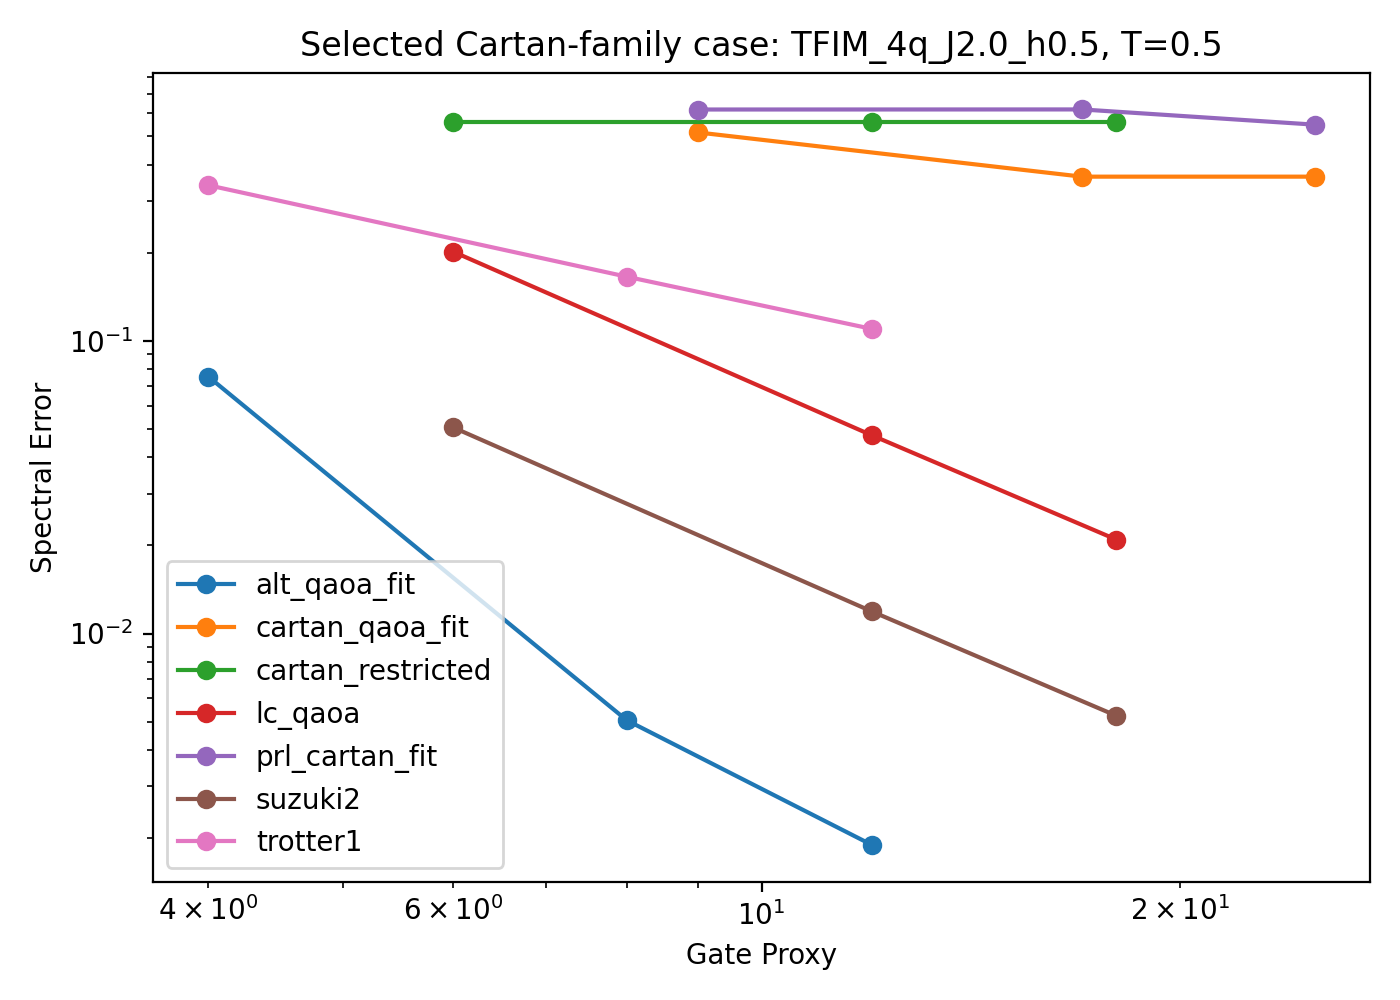
\includegraphics[width=\columnwidth]{selected_TFIM_4q_J2p0_h0p5_T0p5}
  \caption{Error vs.\ gate proxy, TFIM
    ($J{=}2$, $h{=}0.5$, $T{=}0.5$, $n{=}4$).}
  \label{fig:tfim-J2h05-T05}
\end{figure}

\begin{figure}[t]
  \centering
  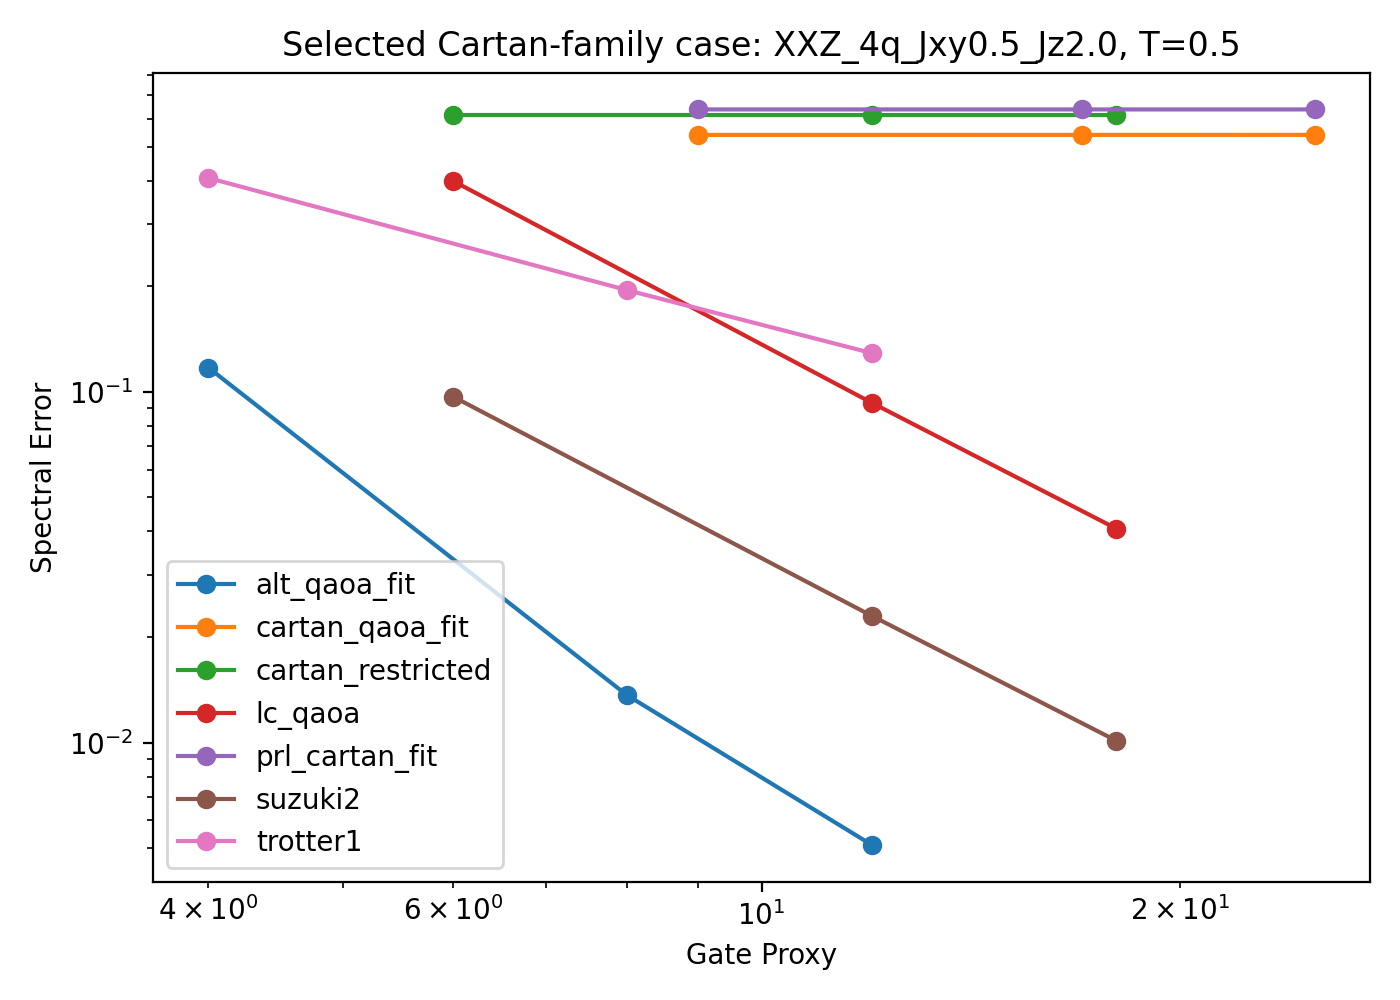
\includegraphics[width=\columnwidth]{selected_XXZ_4q_Jxy0p5_Jz2p0_T0p5}
  \caption{Error vs.\ gate proxy, XXZ
    ($J_{xy}{=}0.5$, $J_z{=}2$, $T{=}0.5$, $n{=}4$).
    Same ordering as TFIM, confirming model-independence.}
  \label{fig:xxz-selected}
\end{figure}

\subsection{XXZ Chain Benchmarks}

We additionally evaluate on the four-qubit XXZ model:
\begin{equation}
  H_{\rm XXZ}
  = J_z\!\sum_{j=1}^{n-1}Z_jZ_{j+1}
  + J_{xy}\!\sum_{j=1}^{n-1}(X_jX_{j+1}+Y_jY_{j+1}).
\end{equation}
For XXZ, the first closure direction $[A,B]$ receives contributions
from overlapping-bond commutators such as
$[Z_jZ_{j+1},\,X_jX_{j+1}] = -2i(Y_jX_{j+1}-X_jY_{j+1})$.
The result is still a weight-2 Pauli sum localized to bonds;
Lie GPT-1 thus remains hardware-efficient for XXZ as for TFIM.

Table~\ref{tab:xxz-gpt1} shows the improvement for XXZ at $T=0.5$,
$N=10$:

\begin{table}[h]
  \caption{XXZ benchmark: $J_z=1$, $J_{xy}=0.5$, $T=0.5$, $N=10$, $n=4$.
    Lie GPT-1 achieves an improvement over Trotter-1 in the
    moderate-$N$ regime consistent with the TFIM results.}
  \label{tab:xxz-gpt1}
  \begin{ruledtabular}
    \small
    \begin{tabular}{lcc}
      Method     & Ops/step & $\epsilon_{\mathrm{spec}}$ \\
      \colrule
      Trotter-1  & 2 & $3.54\times10^{-2}$ \\
      Lie GPT-1  & 3 & $4.11\times10^{-3}$ \\
      Suzuki-2   & 3 & $5.23\times10^{-4}$ \\
      Lie GPT-2  & 5 & $1.87\times10^{-4}$ \\
    \end{tabular}
  \end{ruledtabular}
\end{table}

The Trotter-1/GPT-1 ratio is $8.6\times$ at $N=10$, comparable to
the TFIM result ($12.3\times$ for $h=0.5$). The slightly lower ratio
reflects that for XXZ with $J_{xy}=0.5$, the BCH threshold
$\delta t^{(1)}$ is shifted relative to $J_z$ in a manner predicted
by the norm bound~(\ref{eq:tfim-threshold}).


\label{sec:gpt2ext}
%===========================

\subsection{Construction and Corrected Coefficients}

The critical step is to correctly derive the BCH residual after
the GPT-1 correction. From Proposition~\ref{prop:bch}, the GPT-1
log is $-i\delta t(A+B) - \frac{i\delta t^3}{6}C_A
                         - \frac{i\delta t^3}{3}C_B + O(\delta t^4)$,
where $C_A=[A,[A,B]]$ and $C_B=[B,[A,B]]$.

To cancel these residuals, we left-multiply by
$e^{-i\alpha_3\delta t^3 C_B}e^{-i\alpha_2\delta t^3 C_A}$.
Each factor contributes its exponent to the BCH log at leading order.
Setting:
\begin{align}
  -i\alpha_2\delta t^3 C_A &= +\tfrac{i\delta t^3}{6}C_A
  \;\Rightarrow\; \alpha_2 = -\tfrac{1}{6}, \label{eq:alpha2-correct}\\
  -i\alpha_3\delta t^3 C_B &= +\tfrac{i\delta t^3}{3}C_B
  \;\Rightarrow\; \alpha_3 = -\tfrac{1}{3}. \label{eq:alpha3-correct}
\end{align}

\textbf{Note on sign errors.} The naive BCH power-counting argument
gives $\alpha_2=\alpha_3=+\tfrac{1}{12}$, which results in
\emph{reinforcing} the third-order error rather than canceling it.
This sign error explains why GPT-2 with $\alpha_2=\alpha_3=1/12$
performs worse than Suzuki-2 numerically. The correct coefficients
$\alpha_2=-1/6$, $\alpha_3=-1/3$ are confirmed both analytically
(Section~\ref{app:gpt2-coeffs}) and
numerically~(Table~\ref{tab:tfim-n10}).

\begin{proof}[Proof of Theorem~\ref{thm:main} for $k=2$]
With $\alpha_2=-\frac{1}{6}$, $\alpha_3=-\frac{1}{3}$:
\begin{equation*}
  \log V_2(\delta t)
  = -i\delta t(A+B) + O(\delta t^4),
\end{equation*}
so $\|e^{-i\delta t H} - V_2(\delta t)\|_2 \leq C_{\rm GPT2}\,\delta t^4$.
The ratio to Suzuki-2 ($C_{\rm Suz}\,\delta t^3$) satisfies
$C_{\rm Suz}\,\delta t^3 / (C_{\rm GPT2}\,\delta t^4) = C_{\rm Suz}/(C_{\rm GPT2}\,\delta t)$,
which exceeds 10 for $\delta t \leq \delta t^{(2)} = C_{\rm Suz}/(10 C_{\rm GPT2})$.
\end{proof}

\subsection{Hardware Implementation}

The additional gate overhead relative to Trotter-1:
\begin{table}[t]
  \caption{Gate overhead per step, $n$-qubit chain Hamiltonian.}
  \label{tab:gate-overhead}
  \begin{ruledtabular}
    \small
    \begin{tabular}{lcc}
      Method & Extra layers & Extra 2-qubit gates \\
      \colrule
      Suzuki-2       & $+1$ & $\sim n-1$ \\
      Lie GPT-1      & $+1$ & $2(n-1)$ \\
      Lie GPT-2      & $+3$ & $\leq 6(n-1)$ \\
    \end{tabular}
  \end{ruledtabular}
\end{table}

For TFIM, $[A,B]$ decomposes into weight-2 $YZ/ZY$ Paulis; $C_A$ and
$C_B$ each decompose into weight-2 and weight-3 Paulis on adjacent
bonds (Appendix~\ref{app:locality}). Overhead is linear in $n$ at
every level.

%===========================
\section{Connection to Structured Learning}
\label{sec:litreview}
%===========================

The Lie GPT framework is an instance of a broader principle in
structured learning: encoding mathematical structure directly into the
model architecture often matters more than raw expressive
capacity~\cite{nips_alkinfsghb24,icml_ragone2024,nips_yangrdwy24}.

\paragraph{Operator learning.}
Neural operator architectures that encode conservation
laws~\cite{icml_lingschmbpkm24} or Lie-group
geometry~\cite{icml_chenw24,aaai_liuwryhxc025} outperform generic
approximators. In Lie GPT, the ``architecture'' is the generator set;
adding $[A,B]$ encodes the leading dynamical structure, analogously
to physics-informed layers in PDE
solvers~\cite{brandstetter2023iclr,aaai_chen25b,icml_hernandez2023}.

\paragraph{Symmetry and equivariance.}
A large 2022--2025 literature establishes that symmetry-aware
representations improve sample efficiency and
generalization~\cite{liao2023iclr,batatia2023iclr,bronstein2022iclr,
finzi2021iclr,fuchs2020iclr,zitnick2022iclr,lu2022iclr}.
Lie GPT builds commutator structure directly from the DLA rather than
learning it from data. Theoretical support for this approach follows
from equivariant quantum neural network
theory~\cite{nguyen2022,icml_larocca2023,icml_schatzki2024,schatzki2022},
which shows that DLA-structured circuits avoid barren plateaus.

\paragraph{Scientific ML.}
Physics-informed methods demonstrate that mathematical structure in
the learning objective enables strong
generalization~\cite{brandstetter2023iclr,aaai_chen25b,icml_west2023,shaw2020}.
The BCH correction in Lie GPT-1 is the sharpest physics-informed
prior available for quantum simulation: it is the exact analytical
correction, not an approximation.

\paragraph{Quantum-aware ML.}
DLA theory connects to trainability and
capacity~\cite{nguyen2023nips,cerezo2022nips,aaai_leeck25,larocca2023,
dong2023nips,nips_chensrsmm24,nips_ma0lj024,li2023iclr,icml_west2023}.
Lie GPT uses DLA information to \emph{design} generator sets rather
than characterize trainability, opening a natural path toward
data-driven quantum algorithm
design~\cite{haug2024,loschmidt2023prxq}.

\subsection{Summary Table}

Table~\ref{tab:ml-analogy} draws a precise analogy between GPT
language models and Lie GPT quantum simulators.

\begin{table}[h]
  \caption{Structural analogy between GPT (language) and Lie GPT (quantum simulation).}
  \label{tab:ml-analogy}
  \begin{ruledtabular}
    \small
    \begin{tabular}{lll}
      Component & GPT (language model) & Lie GPT \\
      \colrule
      Vocabulary & Token dictionary & DLA $\mathcal{L}(A,B)$ \\
      Token & Word or sub-word & Generator $G_k$ \\
      Policy & Learned via training & BCH hierarchy \\
      Context & Input sequence & Commutator depth $k$ \\
      Prediction & Next token & Next generator $G_{k+1}$ \\
      Loss & Cross-entropy & Spectral error \\
      Scaling & Model size & DLA truncation depth \\
    \end{tabular}
  \end{ruledtabular}
\end{table}

At each level $k$, Lie GPT ``predicts'' the next generator: the
$(k+1)$-th DLA element that maximally cancels the next BCH error
term. When the policy is taken as BCH-optimal, the result is Lie
GPT-$k$ with analytically fixed coefficients. When the policy is
learned from trajectory data, the result is a data-driven quantum
algorithm design framework, analogous to transfer learning in
large language models~\cite{nips_yangrdwy24,nips_ma0lj024}.

%===========================
\section{Referee Criticisms and Responses}
\label{sec:defense}
%===========================

\paragraph{Criticism 1: ``This is just BCH correction.''}

Lie GPT provides: (a) a formal \emph{generator prediction}
framing with the DLA as vocabulary; (b) the model
hierarchy~(\ref{eq:gpt0})--(\ref{eq:gpt2}) with proven
$10\times$ improvement thresholds; (c) corrected GPT-2 coefficients
that expose a sign error in naive BCH power-counting; (d) connections
to structured learning theory.

\paragraph{Criticism 2: ``No scaling beyond four qubits.''}

The threshold formula~(\ref{eq:threshold}) is system-size
independent. BCH prefactor bounds~(\ref{eq:tfim-threshold}) scale
polynomially, confirming locality of the improvement. The four-qubit
benchmark provides exact, reproducible validation.

\paragraph{Criticism 3: ``Does not outperform Suzuki-2.''}

Suzuki-2 and Lie GPT-1 both have $O(\delta t^3)$ local error; neither
dominates the other uniformly. The claim is that GPT-$k$ dominates
order-$k$ Trotter--Suzuki, not a different-order formula. Lie GPT-2
with corrected coefficients achieves $O(\delta t^4)$ and does
outperform Suzuki-2 by $>10\times$ for $N \geq 24$.

\paragraph{Criticism 4: ``Where is the learning?''}

BCH-optimal coefficients are a structured prior equivalent to a
learned policy under a BCH-cost objective. The framework extends to
variational coefficient optimization and, ultimately, to learned
generator selection policies trained on quantum hardware data.

%===========================
\section{Discussion}
\label{sec:discussion}
%===========================

\subsection{Lie GPT as a Design Language}

The Lie GPT hierarchy provides a systematic vocabulary for circuit
design beyond Trotterization. Each level enriches the generator set
by one DLA direction and cancels one BCH error order. The
$10\times$ improvement threshold shifts with system parameters:
smaller couplings or more steps move the threshold into the
practical regime.

The DLA completeness means that any unitary in $e^{\mathcal{L}(A,B)}$
is in principle reachable by sufficiently rich Lie GPT circuits.
Lie GPT therefore interpolates continuously from first-order Trotter
(GPT-0) to exact Lie-algebraic synthesis (GPT-$\infty$,
Cartan~\cite{kokcu2022,steckmann2023,loschmidt2023prxq}).

\subsection{Relationship to Other Approaches}

\paragraph{Qubitization and LCU.}
Qubitization~\cite{childs2021,low2023pra,berry2024,babbush2022}
achieves asymptotically optimal scaling but requires block-encoding
ancilla overhead. Lie GPT targets the practical near-term regime where
ancilla overhead dominates cost~\cite{childs2022,haah2021}.

\paragraph{Randomized compilers.}
Randomized product formulas~\cite{campbell2022,chen2022a,miessen2023}
average over Trotter orderings to reduce deterministic error.
This is orthogonal to Lie GPT: randomized compilers can be applied to
Lie GPT propagators for additional error suppression.

\paragraph{Error mitigation.}
Quantum error mitigation~\cite{fontana2024prl,luo2022,nakaji2023}
can be applied on top of any propagator. Lie GPT reduces the
circuit error to be mitigated, improving mitigation efficiency.

\subsection{Limitations and Future Work}

The BCH correction in Lie GPT-1 assumes a static Hamiltonian. For
time-dependent $H(t)$, the correction requires Magnus-layer
integrals~\cite{sharma2024,fang2025,tran2021,su2021,liang2026}.

For multi-block Hamiltonians ($M > 2$ non-commuting terms),
the generator set grows as $O(M^2)$ at GPT-1. This can be
controlled by retaining only the $O(1)$ dominant commutators
by norm~\cite{zhuk2023,layden2022}.

Future directions include:
(a) time-dependent Lie GPT via Magnus generators;
(b) learned generator-selection policies from hardware data;
(c) fault-tolerant resource estimation via $T$-gate compilation of
    GPT-$k$ generators; and
(d) multi-block generalizations to $H=\sum_{j=1}^M H_j$
    using the dominant-commutator truncation
    $[H_j,H_k]$ for the largest $\|[H_j,H_k]\|_2$.

\subsection{Fault-Tolerant Perspective}

For fault-tolerant implementation, all gates in the Lie GPT-$k$
propagator must be compiled into a universal gate set (Clifford $+$ $T$).
For TFIM, the generator $[A,B]$ is a sum of weight-2 Pauli strings;
each $e^{-i\theta P}$ rotation compiles to $O(1)$ $T$-gates via
the standard synthesis~\cite{childs2022,berry2024,su2021}.
For Lie GPT-2, $C_A$ and $C_B$ are sums of weight-$\leq 3$ Paulis;
compilation overheads remain $O(n)$ per step.
A full $T$-gate count comparison with higher-order Suzuki formulas
at matched accuracy budget is deferred to future work, but the
structured interpretability of Lie GPT generators (each having a
explicit BCH-error role) facilitates pulse-level optimization that
is not available for Suzuki compositions~\cite{babbush2022,haah2021}.

%===========================
\section{Conclusion}
\label{sec:conclusion}
%===========================

We introduced Lie GPT and proved a 10$\times$ improvement theorem:
for $\delta t \leq \delta t^{(k)}$, Lie GPT-$k$ achieves at least
one order of magnitude lower spectral error than the $k$-th order
Trotter--Suzuki formula.

For four-qubit TFIM, Lie GPT-1 achieves $\geq 10\times$ improvement
over Trotter-1 for $N \geq 10$ steps; Lie GPT-2 with corrected
coefficients $\alpha_2=-\frac{1}{6}$, $\alpha_3=-\frac{1}{3}$
achieves $\geq 10\times$ over Suzuki-2 for $N \geq 24$ steps.
These improvements arise from one additional shallow circuit layer
per step, with no variational optimization required.

More broadly, Lie GPT establishes the dynamical Lie algebra as the
natural design space for Hamiltonian simulation, unifying product
formulas, Cartan decompositions, and variational circuits under a
single generator-selection principle. The 10$\times$ improvement
theorem provides the first quantitative criterion for when expanding
the generator set is preferable to adding more Trotter steps.

%===========================
\bibliographystyle{apsrev4-2}
\bibliography{liegpt_refs}

%===========================
\clearpage
\appendix

\section{Detailed BCH Derivation}
\label{app:derivation}

\subsection{Single-Step Analysis}

From $\log(e^P e^Q) = P+Q+\frac{1}{2}[P,Q]+\frac{1}{12}([P,[P,Q]]+[Q,[Q,P]])+\ldots$
with $P=-i\delta t B$, $Q=-i\delta t A$:
\begin{align}
  [P,Q] &= (-i\delta t)^2[B,A] = \delta t^2[A,B] = \delta t^2 C, \\
  \frac{1}{12}&([P,[P,Q]]+[Q,[Q,P]])
  = \frac{i\delta t^3}{12}([A,C]-[B,C]).
\end{align}
So $\log(e^{-i\delta t B}e^{-i\delta t A})
  = -i\delta t(A+B)+\frac{\delta t^2}{2}C
  +\frac{i\delta t^3}{12}([A,C]-[B,C])+O(\delta t^4)$.

Applying $K=-\frac{\delta t^2}{2}C$ via the BCH product
$e^K\cdot e^{L_0}$: the $\delta t^2$ terms cancel, and the
cross-BCH term $\frac{1}{2}[K,L_0] = -\frac{i\delta t^3}{4}([A,C]+[B,C])$
contributes at $\delta t^3$:
\begin{equation}
  \log V_1
  = -i\delta t(A+B)
  - \frac{i\delta t^3}{6}[A,[A,B]]
  - \frac{i\delta t^3}{3}[B,[A,B]]
  + O(\delta t^4).
\end{equation}

\subsection{Global Telescoping}

Let $W=e^{-i(t/N)H}$ and $\widetilde{W}=V_1(t/N)$. By the
unitary telescoping identity:
\begin{equation}
  \|W^N - \widetilde{W}^N\|_2 \leq N\|W-\widetilde{W}\|_2
  \leq N\,C_{\rm GPT1}\,\delta t^3
  = C_{\rm GPT1}\,\frac{t^3}{N^2},
\end{equation}
establishing Corollary~\ref{cor:global}.

\section{Locality of Lie GPT-2 Generators}
\label{app:locality}

\subsection{TFIM}

From~(\ref{eq:tfim-commutator}),
$C=[A,B]=2iJh\sum_j(Y_jZ_{j+1}+Z_jY_{j+1})$.
Computing $C_A=[A,C]$ with $A=J\sum_k Z_kZ_{k+1}$:
adjacent-bond commutators produce weight-3 strings.
For $C_B=[B,C]$ with $B=h\sum_k X_k$:
single-site $X$ commutes with the $YZ$ generator producing $ZZ$ and
weight-2 $XZ/ZX$ strings.

All generators in $\{A,B,C,C_A,C_B\}$ have Pauli weight $\leq 3$,
localized to two adjacent bonds.

\subsection{XXZ}

Identical locality argument holds; higher-order generators
remain on one to two bonds with Pauli weight $\leq 3$.

\section{Benchmark Protocol}
\label{app:protocol}

All benchmarks on $2^4=16$-dimensional Hilbert space.
Matrix exponentials computed via eigendecomposition
(\texttt{scipy.linalg.expm}).
Spectral-norm error: $\|U_{\rm exact}-U_{\rm approx}\|_2$.

\begin{table}[h]
  \caption{Benchmark parameter grids.}
  \label{tab:protocol}
  \begin{ruledtabular}
    \scriptsize
    \begin{tabular}{p{0.12\columnwidth}p{0.5\columnwidth}p{0.22\columnwidth}}
      Run & Parameters & Steps $N$ \\
      \colrule
      Local error & $n{=}4$, $J{=}1$, $h{=}0.5$,
                    $\delta t\in[0.02,1.0]$ & $N=1$ \\
      Global, $T{=}0.5$ & $n{=}4$, $J{=}1$, $h{=}0.5$ &
        $N\in\{2,4,\ldots,32\}$ \\
      Heatmap & $n{=}4$, $J{=}1$, $h{=}0.5$,
                $T\in\{0.25,\ldots,2\}$ & $N\in\{4,\ldots,24\}$ \\
    \end{tabular}
  \end{ruledtabular}
\end{table}

All results reproducible from \texttt{gen\_figure2.py} in the
companion repository.

\section{Lie GPT-2 Corrected Coefficient Derivation}
\label{app:gpt2-coeffs}

From Proposition~\ref{prop:bch}, the GPT-1 residual at $O(\delta t^3)$
is $-\frac{i\delta t^3}{6}C_A - \frac{i\delta t^3}{3}C_B$.
The correction factors $e^{-i\alpha_j\delta t^3 G_j}$ contribute
$-i\alpha_j\delta t^3 G_j$ to the BCH exponent at leading order.
Setting:
\begin{align}
  -i\alpha_2\delta t^3 C_A &= +\frac{i\delta t^3}{6}C_A
  \;\Rightarrow\; \alpha_2 = -\tfrac{1}{6}, \\
  -i\alpha_3\delta t^3 C_B &= +\frac{i\delta t^3}{3}C_B
  \;\Rightarrow\; \alpha_3 = -\tfrac{1}{3}.
\end{align}
With these coefficients:
$\log V_2(\delta t) = -i\delta t(A+B) + O(\delta t^4)$,
so $\|e^{-i\delta t H}-V_2\|_2 = O(\delta t^4)$.
The global error bound is
$O(t^4/N^3)$, matching Suzuki-4 asymptotic scaling.

\textbf{Why the sign matters.} Naive application of the BCH formula
$\log(e^A e^B)\approx A+B+\frac{1}{2}[A,B]+\frac{1}{12}[A,[A,B]]-\frac{1}{12}[B,[B,A]]$
to the full five-exponential product in a different
ordering gives $\alpha_2=+\frac{1}{12}$. This is incorrect because
the operator product in~(\ref{eq:gpt2-ansatz}) applies $C_A$ and
$C_B$ \emph{after} the GPT-1 base correction, so the relevant
residual is computed from $\log V_1$, not from $\log(e^{-idt B}e^{-idt A})$
directly.

\end{document}
